



\subsection{Municipal costs and revenue}

\begin{figure}
\begin{center}
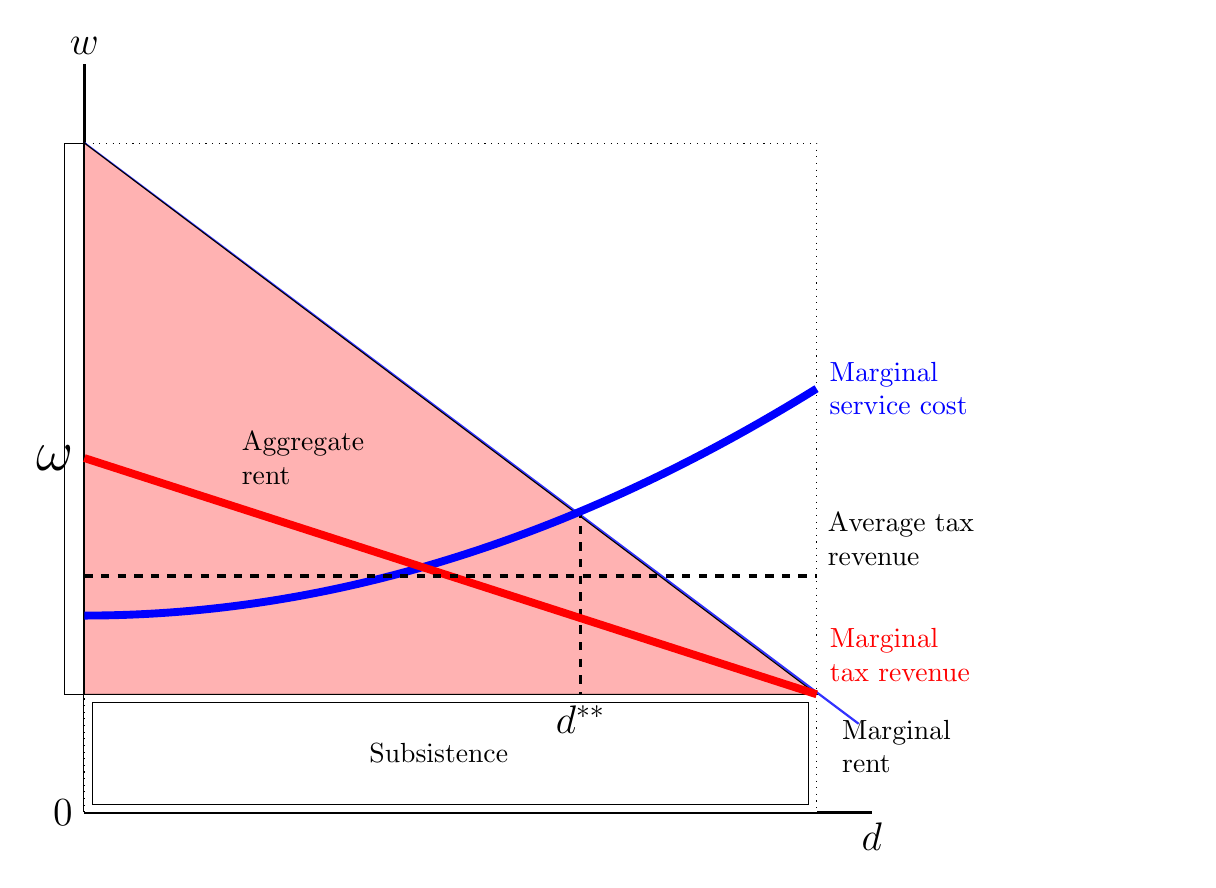
\begin{tikzpicture}[scale=1]
\def\bndmax{5}        %https://tex.stackexchange.com/questions/68462/filling-a-complex-region-with-tikz
\def\bndmin{0.2}
\def \n {8}  % height of y axis
\def \d {10}  % length  of x axis
\def \t {.75}  %  cost of transportation per unit x
\def \th {1}   %
\def \w {7}    %  wage premium
\def \om{1.5}%  omega =rural wage Zero for urban population
\def \azero{2}
\def \aprime {-.0}	
\tikzset{func/.style={thick,color=blue!80}}	
\draw [thick] (0,-\om) --(\d,-\om)node[below]{\Large $d$};  			% Zero for rural population
\draw [thick] (0,-\om)node[left=.5]{\Large $0$} --(0,\n)node[above]{\Large $w$};	% Y axis

%\draw [thick] (0,0)node[left=.5]{ subsistance}--(\d,0);
\node[left=.25] at (0,3){\huge $\omega$};
%\node[left=.25] at (0,\w+.3){subsistence plus};
%\node[left=.25] at (0,\w-.4){wage premium};	

\draw[fill=white, white] (0.1,-0.1) rectangle (14,-\om+.1);
\draw [] (-.25, 0) rectangle(.25, \w);%fill=green!30!blue!30
\node[right] at  (.25, \w/2){Added Productivity};
%\draw [ thick, ->](11.3,-\om/2)--(13, -\om/2)node [right] {\Large $d$};
\draw[fill=blue!40] (0.1,-0.1) rectangle (9.2,-\om+.1);

\draw[fill=black!0, dotted] (0,-\om) rectangle (9.30,\w);% new product repeat
\draw[func, domain=0:\w/\t+.5] plot [samples=200] (\x,{\w-\t*\x}); %rent profile
\draw[fill=blue!0] (0.1,-0.1) rectangle (9.2,-\om+.1);
\node at (4.5,-\om/2){Subsistence};
\draw[fill=red!30,] (0.,0.)--(0,7)--(9.30,0.)--cycle;% Rent \w-.2
\node[text width=2cm] at (3.,3){Aggregate \\rent}; 		%Rent 
%\node at (5.8,5.7)[]{\Large Transportation};
\node at (6.3,4.8)[white]{\Large expenditure};
\draw[ line width=.5mm, dashed] (6.3,2.35)--(6.3,0)node[below ]{\Large $d^{**}$};

\draw[func, domain=0:9.3, line width=1mm,blue, text width=2cm] plot [samples=200] (\x,{1+\x^2/30})node[right]{Marginal\\ service cost};
\draw[ line width=1mm, red] (0,3)--(9.3,0)node[above right, text width=3cm ]{Marginal\\tax revenue};
\node at (9.5, -.2)[below right, text width=2cm]{Marginal rent};

\draw[ line width=.5mm, dashed] (0,1.5)--(9.3,1.5)node[above right, text width=2.5cm ]{Average tax revenue};
%GRID
%\draw[step=1cm,gray,very thin] (0,0) grid (10,10);
\end{tikzpicture}
\end{center}
\caption[The Alonso model with municipal costs and revenue.]{The Alonso model \gls{rent profile}, as illustrated in Figure~\ref{fig-alonso-simple}, with cost and municipal costs and revenue added.} %service fees added.}
\label{fig-municipal-costs}
\end{figure}
 

 Two stylized facts should be noticed. The first is that the marginal cost of servicing generally rises with the distance from the centre. Figure illustrates the general form of servicing costs, but not the relative scales of rent and servicing costs. When this observation is combined with the \gls{Henry George Theorem} the conclusion is that the optimal size of the city  is at  $d^{**}$, where marginal service cost intersects with the marginal increase in total urban rent.  Walter Christaller, 1933

The second stylized fact is that property taxes, which are generally  fixed as a share of property value, decline as the distance from the centre increases. Figure~\ref{fig-municipal-costs} illustrates the general form of tax liabilities, although it does not  accurately represent their relationship to rent or  servicing costs. This implies that in many or most urban situations the residents at the outer edges pay less than the average amount in property tax per unit of land, but cost  the community budget more than the average amount. In essence, the central city subsidizes the suburbs. (see Perverse Cities \ref{blaisPerverseCitiesHidden2011}). This arrangement is both economically inefficient and unfair, but it has been built into the fiscal structure of cities largely as a result of automobile-based urban growth. It is likely that this fiscal misallocation saps some of the potential productivity growth of cities. Property taxation reduces the market value of properties, but it also funds services and amenities that increase the value of properties. 

Both servicing and taxation effects are more variable and than the simple model suggests.  One conclusion urban theorists draw based on variants of the Alonso model is that because property owners in the low-density urban margin are subsidized,  the subsidy is likely to create serious fiscal problems for municipalities in the long-term and result in serious inefficiency in land use.

Political opposition is essentially rent seeking.



% % TEMP - here are some other notes we may want to reference or bring in. [[non individualistic modeling of agents]] [[generalizability in agent vs classical econ models]]